% !TEX root = BusSim.tex
% 
\section{Research problem and related works} \label{s:problem}

Historical and real-time bus GPS data is often used by operators to locate buses and predict their locations and arrival times. For instance, Public Transport Information and Priority System (PTIPS) is a state-of-the-art system in Australia to give priority to public transport vehicles on the roads and provide information on predicted bus arrival to passengers. The prediction of bus locations and arrival times in real time is a challenging problem \citep{chien2002dynamic}. Ideally, perfect 
knowledge of the current state of the system and any underlying processes is required.  However, obtaining this level of knowledge is impossible due to sources of uncertainty and the complex interactions in
bus operations. The majority of research within this area has focused on machine learning methods to find a direct mapping between input
data and bus arrival time. Examples of these methods include Artificial
Neural Networks \citep{chien2002dynamic}, Support Vector Machines
\citep{bin2006bus}, and Bayesian techniques
\citep{khosravi2011prediction}. While machine learning methods are generally
efficient in real time, they are solely reliant on the quality of available
data. Even with high-resolution datasets that record accurate spatio-temporal bus locations, the full complexity of the system will never be captured. 

%Without an understanding of the underlying processes driving bus operation, these models fail to quantify uncertainty and will perform poorly in highly stochastic systems, in unseen situations or when data are missing.

There are analytical and simulation models of bus routes that aim to
reproduce the underlying processes in bus operations, and shed some
light on the associated uncertainties. One of the earliest successes in simulating a simple bus systems was from Cellular Automata modelling
\citep{luo2012realistic,o1998jamming,chowdhury2000steady,
jiang2003realistic}. Whilst the dynamical foundations of these models
are well understood, they are outperformed by more sophisticated
models such as bus-following models
\citep{nagatani2000kinetic,huijberts2002analysis,Tang2012,
nagatani2001bunching,hill2003numerical}; and traffic-following models
\citep{cats2010mesoscopic,toledo2010mesoscopic,hans2015real}.
Bus-following models aim to model the fundamental dynamics of a bus
route by modelling individual buses that follow each other (for example speeding up if the bus ahead is far away). Traffic-following models,
on the other hand, aim to model buses as a component of a transport
system with private and public transport, where their speeds are
affected by the traffic flow, traffic signals \citep{hans2015real} or
traffic density \citep{toledo2010mesoscopic}.

The majority of these models are \textit{static}, i.e. they only have parameters that are fixed over time. We can represent these static simulators 
with the equation $Y = f(X)$, where $f$ represents the simulator. A run of a simulation is defined
as the process of producing one set of data $Y$ for a single set of
model parameters $X$. One way for these
models to reduce their uncertainty and fit more closely to the observed data is to
adjust the model parameters until the model satisfies some predetermined
criteria. This parameter adjustment process is often referred to as
\textit{parameter calibration}. Popular optimisation techniques include simulated annealing~\citep{pennisi_optimal_2008}, genetic
algorithms,~\citep{heppenstall_genetic_2007, malleson_optimising_2014},
and approximate Bayesian computation~\citep{grazzini_bayesian_2017}.
Parameter calibration, especially with ABMs, is often only
implemented once, and therefore cannot account for any changes that may take place within
the system. In the traffic context these might include accidents, traffic signal failures, vehicle faults, etc. Static models are simple to implement, but struggle to model dynamic systems. 


%Many advanced simulators are now \textit{dynamic}: they have inputs and
%outputs that vary over time and operate iteratively over fixed
%time steps. A real bus route is an example of a dynamic system, where
%the arrival rate of passengers and the surrounding traffic vary across
%different times of day, days of the week, and even seasonally. A dynamic
%simulator may be written in the form $Y_t = f(X_t)$, where $Y_t$ is the
%set of outputs at time $t$ and $X_t$ subsumes both fixed model
%parameters and time-varying variables at time step $t$. 

In real-time applications, e.g bus location or bus arrival time prediction in real time, prediction models often have to deal with the fact that there are so much uncertainty in bus operations. Real bus operation is \textit{dynamic} (changing over time) and also \textit{stochastic} (contains inherent randomness). In real time, there are also many unobservable information of bus operation, such as the number of passengers who are waiting at
downstream stops or the number who plan to get off the bus, and the
surrounding traffic conditions.  The lack of information about these factors means that any model of bus
operation in real time will have to make assumptions thereby introducing uncertainties. 

Therefore, this research will explore a combination of parameter calibration and a \textit{data
assimilation} (DA) technique to calibrate a dynamic ABM bus route simulator using historical data, and then dynamically optimised it on-the-fly using real-time data. This, in itself, is a novel and important
contribution. Few previous efforts have attempted to incorporate data
assimilation with agent-based models \citep[for example
see][]{ward_dynamic_2016, wang_data_2015}, and it is unclear how DA
methods, that have typically been created for linear models
\citep{harvey1990forecasting}, can be adapted for non-linear ABMs. 

DA methods assume that observational data are sparse and only describe
the target system in limited detail. Therefore a model is essential as a
means of filling in the gaps in space and time left by the observations through the generation of additional data.
In effect, the model propagates data from observed to unobserved areas
\citep{carrassi_data_2018}.  Although techniques can be used to
perform parameter estimation, they are most often framed as a state
estimation problem. The aim is to calculate a posterior probability for
the state vector $X_t$, given prior distributions from a model (in this
case, a bus route operation model) and data from observations. It is
this marriage of a model and real-time observational data (and the 
associated uncertainties) that offers the means of allowing all the
available information to be used to determine the true state of the
system as accurately as possible \citep{talagrand_use_1991}.

Models where the system state at time $t$ are only dependent on the state at time $t-1$ are termed \textit{Markovian}. We are particularly interested in ABMs that can be written in a Markovian nature because DA algorithms require knowledge to the \textit{full} model state in the form of the state vector $X_t$. While some ABMs in the literature track agent histories and use this information to decide future states, these can be recast as Markovian ABMs by expanding the state vector to include these histories. Implementing a bus route system as a Markovian model requires variables such as vehicle locations, speeds, occupancies etc. It is reasonable to
assume that the system state at the next time step only depends on the
value of these variables at the current time step. For simplicity, we
assume that the state vector used here has a fixed size.  The unused variables (i.e. those for buses that have yet to enter the system) can be set to zero, enabling the state vector to be treated as sparse and
passed efficiently between iterations. If the state vector has a fixed
size, then all possible states of the system belongs to a state-space
$\mathcal{X} \in \mathbb{R}^n$. The system state evolves in some fixed
interval \{0,..,K\}. We denote the state of the bus route at time $t$ by
$X_t \in \mathcal{X}$.

This paper follows an `identical twin' experiment framework \cite{wang_data_2015}, where experiment data to be used will be generated from simulation, instead of using real data. The reason is that real data often comes with noise that hides the true state of the bus route (e.g. noise from GPS data). A simulated synthetic data would enable us to control the level of noise in the data, and to evaluate the modelling results against the ground truth rather than noisy data. Figure \ref{fig:workflow} shows the workflow of this study. 

\begin{figure}[H]  \centering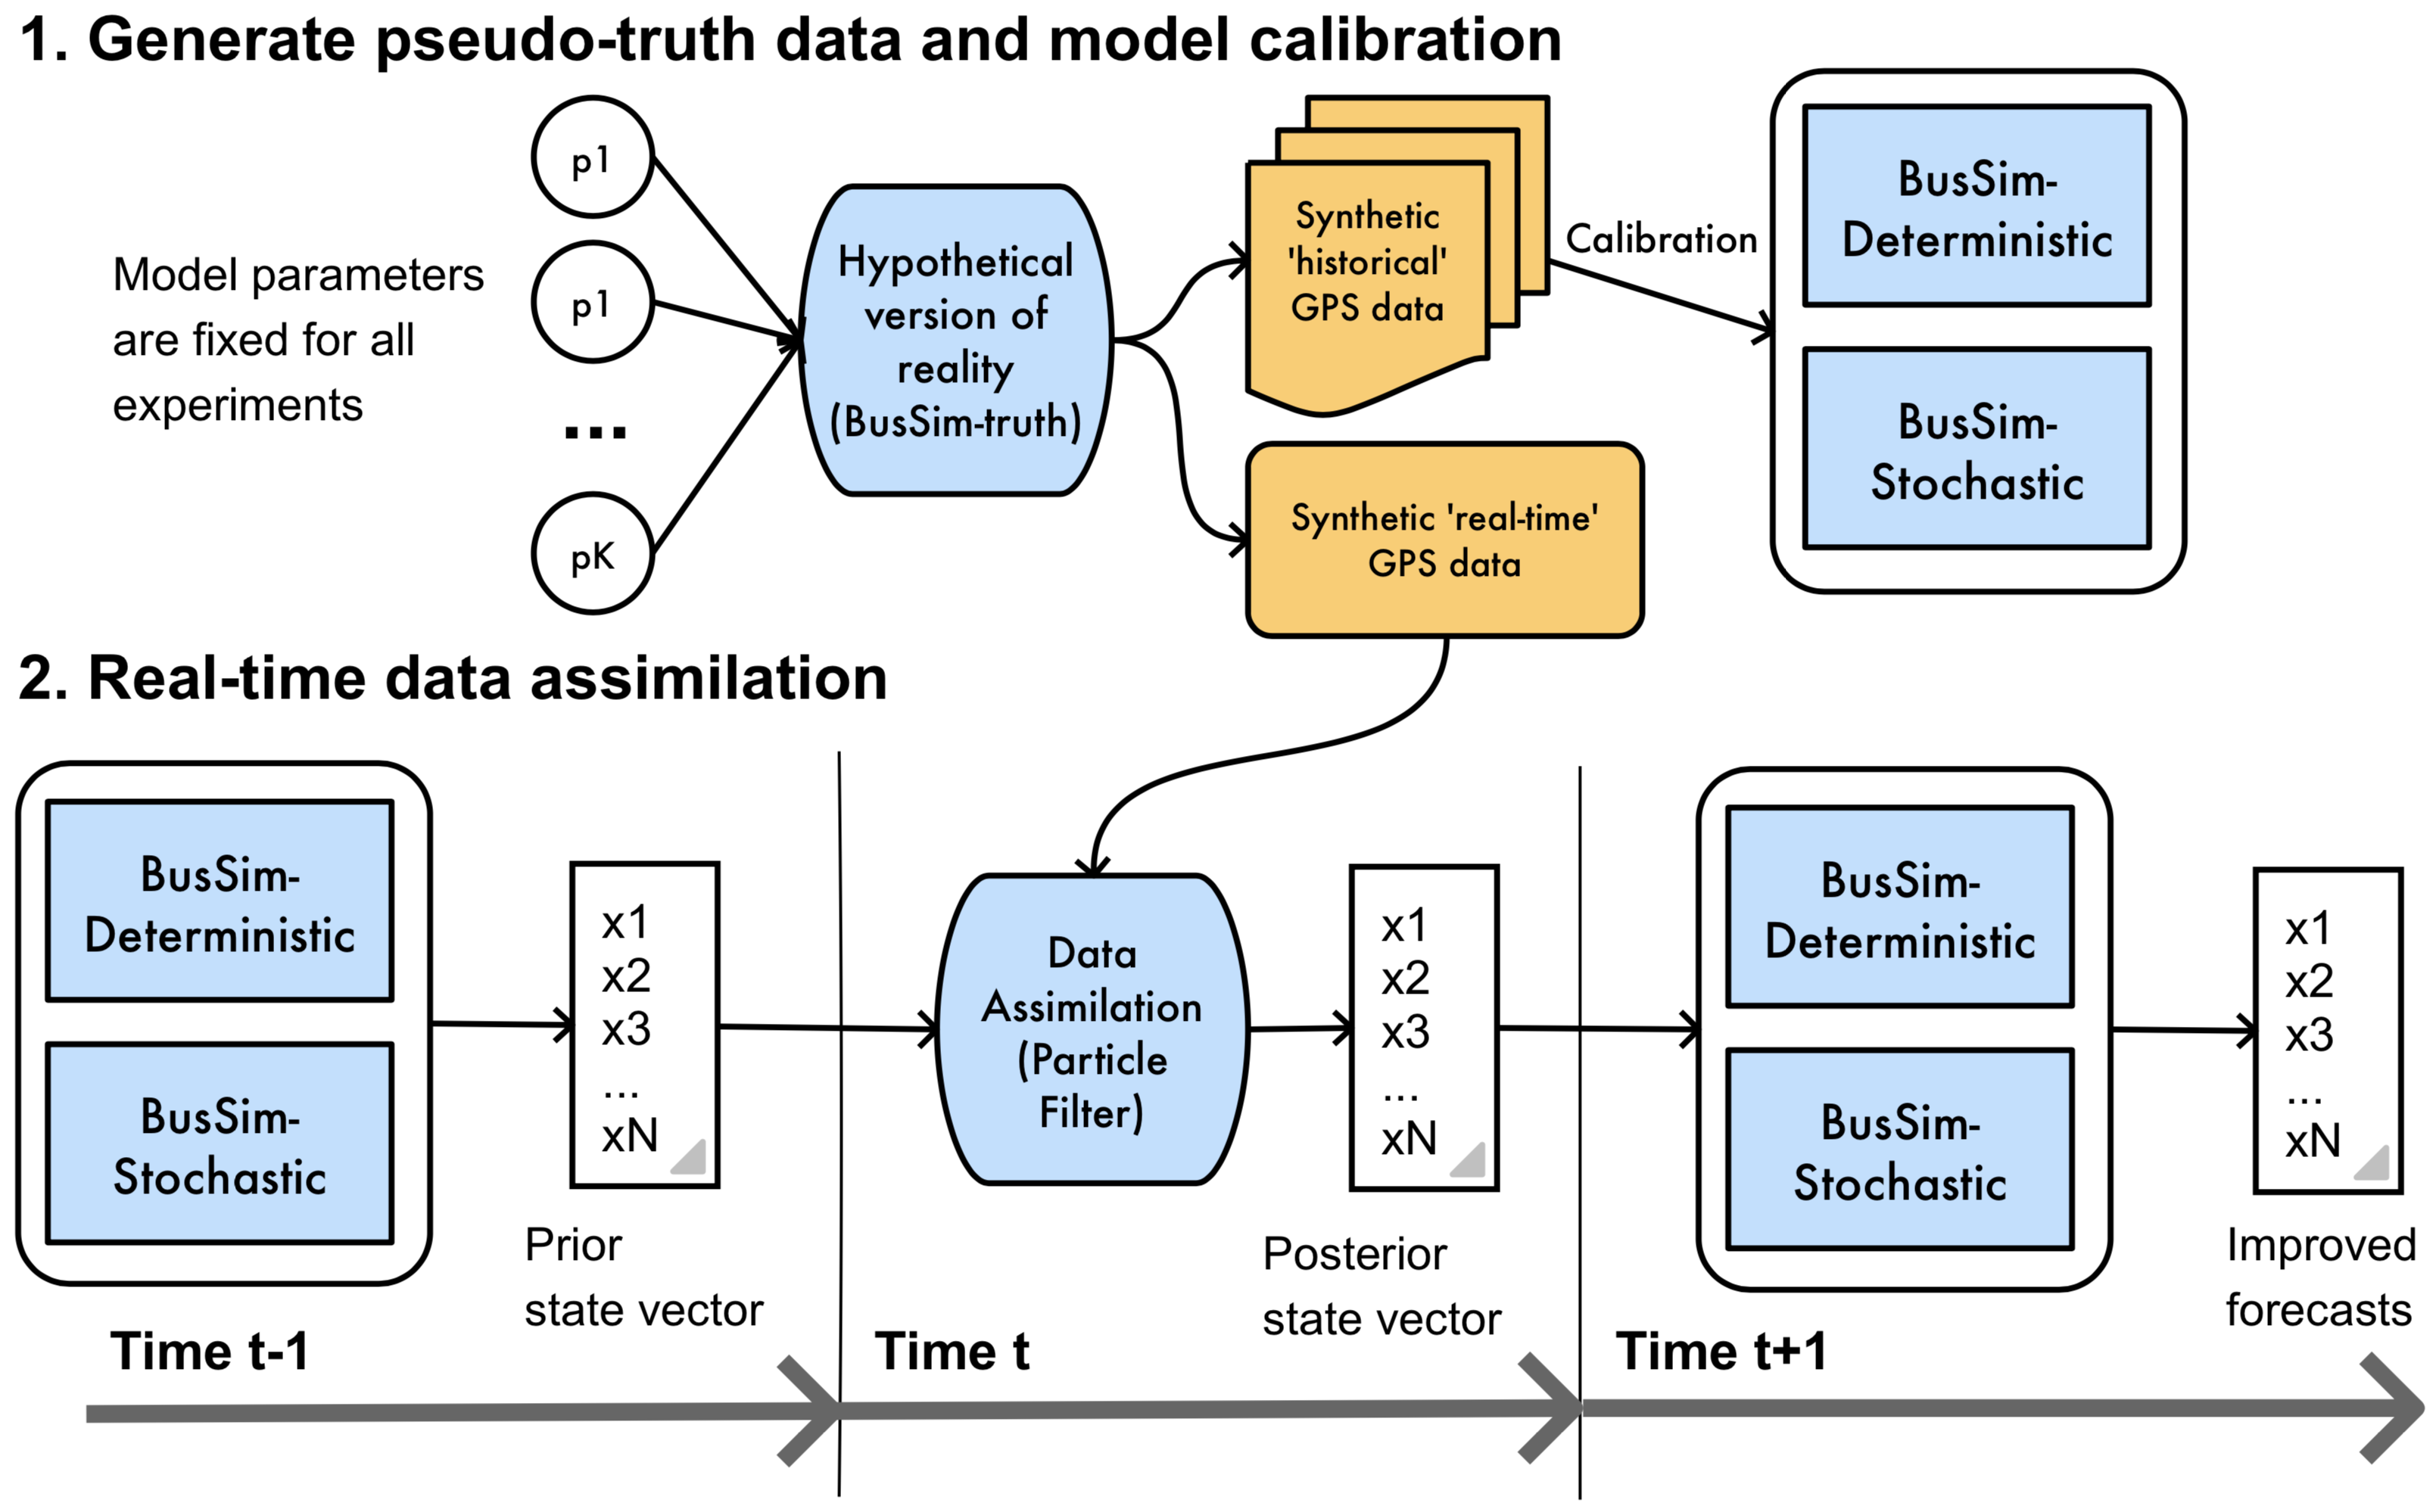
\includegraphics[width=13cm]{Figures/bussim-framework.png}
\caption{Study workflow.} 
\label{fig:workflow} 
\end{figure}

The study workflow generally consists of 2 major steps. It starts with the development of a Markovian ABM of bus route operation that will be referred as \textit{BusSim-truth}. BusSim-truth is a hypothetical version of reality and will be used to generate synthetic GPS data of bus locations with timestamps. Two sets of data will be generated. The first represents `historical' GPS data, which are essentially the outputs of multiple runs of the same BusSim-truth model with the same predefined set of parameters. The GPS data will be slightly different each time the model is run because BusSim-truth is stochastic (its outputs vary slightly from one run to another) and dynamic (the parameters that control factors such as the amount of traffic vary during a single model run). The second set of data represent a single run of BusSim-truth, also using the same set of parameters. These data will represent synthetic `real-time' GPS data and will be used to conduct data assimilation. This situation is similar to the reality, where `historical' data across multiple days are used to calibrate models and `real-time' data represent the \textit{current} state of the world. BusSim-truth will be reasonably realistic and will replicate popular phenomenon in bus operations such as bus bunching (two buses of the same line arrive at the same bus stop at the same time). 

In reality, any simulation model is a simplification of the actual dynamics. Taking this into consideration, we develop two simpler variations of BusSim-truth, knowing that they would not be able to perfectly represent the dynamics in BusSim-truth.  The two variations are: 
\begin{itemize} 
	\item \textbf{BusSim-deterministic}. This model evolves exactly the same way in each model run;
	\item \textbf{BusSim-stochastic}. This model is stochastic, e.g. the numbers of people waiting at bus stops is drawn from a random distribution 
\end{itemize} 

As would be necessary in reality, BusSim-deterministic and BusSim-stochastic will first be calibrated against the synthetic `historical' GPS data. In the second step of the study workflow, DA will be used in an attempt to update the states of the models to the `real-time' GPS observations in order to produce more accurate short-term forecasts of the system behaviour. 
